% Benchmark Evaluation Section

Benchmark Evaluation

\subsection{Methodology}
\label{subsec:methodology}

\begin{table*}
\caption{Benchmark System Configurations}
\label{tab:benchsys}
\begin{tabular}{cccccccc}
\toprule
System&Clock&Threads/Socket&Sockets&Cache/Socket&MemSize&OS&Compiler\\
\midrule
Xeon-X5650&2.67Ghz&12&2&12MiB&64GiB&Ubuntu 18.04 4.15.0-88 & GCC 7.5.0\\
Xeon-E5620&2.4Ghz&8&2&12MiB&48GiB&Ubuntu 16.04 4.4.0-87 & GCC 5.4.0\\
Core i5-3210M&2.5Ghz&4&1&3MiB&4GiB&macOS 10.13.6&clang 9.1.0\\
Opteron 4130&800Mhz&4&2&512MiB&64GiB&Centos7 3.10.0-957.12.1&GCC 8.3.1\\
Cortex-A72&1.5Ghz&4&1&1MiB&4GiB&NNN&NNN\\
Cortex-A53&1.4Ghz&4&1&64KiB&512MiB&NNN&NNN\\
Xeon-E5-2620&2.4Ghz&12&1&15MiB&64GiB&Ubuntu 16.04 4.4.0-164&GCC 5.4.0\\
Xeon-E5-2670&2.5Ghz&10&2&25MiB&64GiB&Centos7 3.10.0&GCC 7.3.0\\
Xeon-E5-2695&2.1Ghz&36&2&45MiB&192GiB&Centos7 3.10.0&GCC 7.3.0\\
i7-3930K&3.2Ghz&12&1&12MiB&64GiB&Linux Mint 18.3 4.15.0-46&GCC 5.4.0\\
i7-4980HQ&2.8Ghz&8&1&6MiB&16GiB&macOS 10.15.3&GCC 9.2.0\\
Ryzen V1605B&1.4Ghz&8&1&512KiB&32GiB&Ubuntu 19.04 5.2.10&GCC 8.3.0\\
Xeon Phi 7250&1.4Ghz&272&1&1MiB&96GiB&SLES 4.12.14&GCC 8.3.0\\
Xeon E5-2698&2.3Ghz&32&2&40MiB&128GiB&SLES 4.12.14&GCC 8.3.0\\
\bottomrule
\end{tabular}
\end{table*}

\todo{Notate disabled SMT on Xeon E5-2670??, 4980hq crystalwell cache, phi 7250 - 16GB HMC/MCDRAM + 1MB x 34 cache}

\subsection{Results}
\label{subsec:results}

\begin{figure}[!t]
\centering
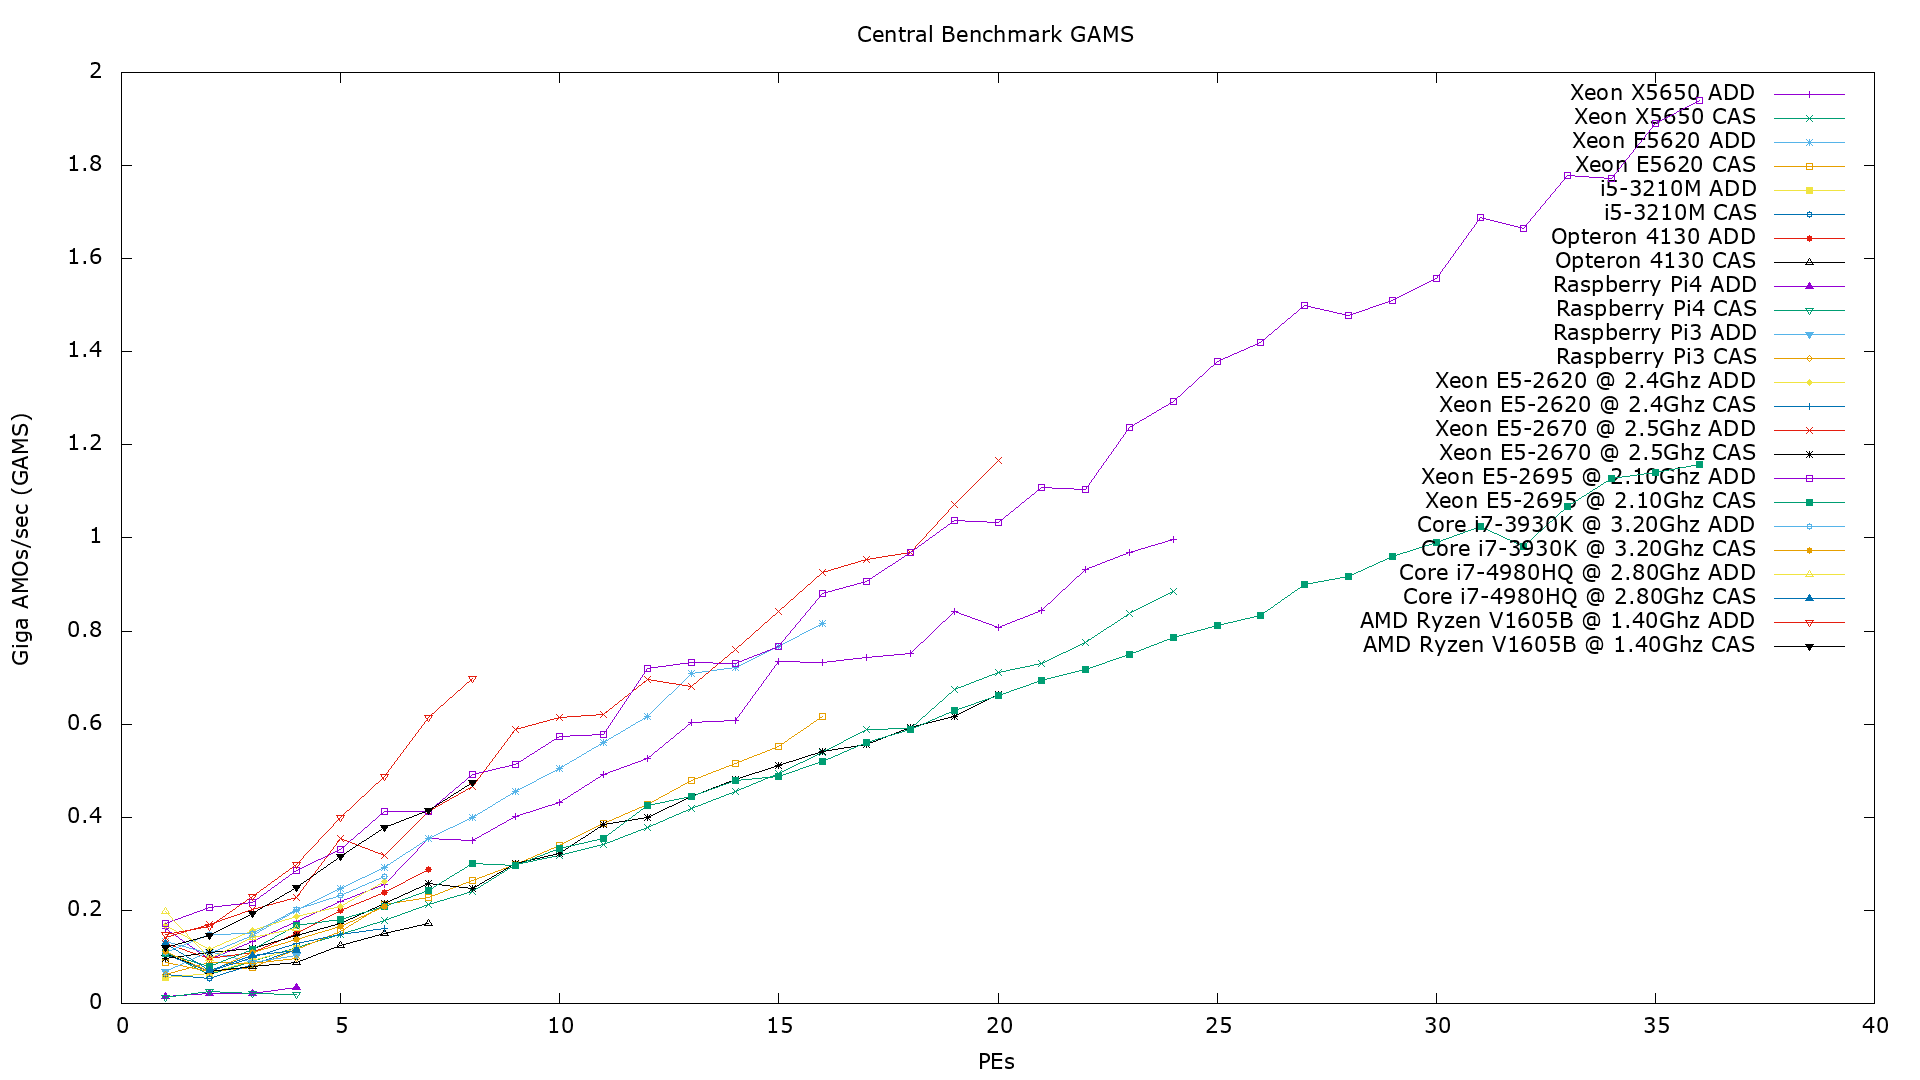
\includegraphics[width=3.5in]{figures/CENTRAL_GAMS.png}
\caption{Central Benchmark GAMS}
\label{fig:central_gams}
\end{figure}

\begin{figure}[!t]
\centering
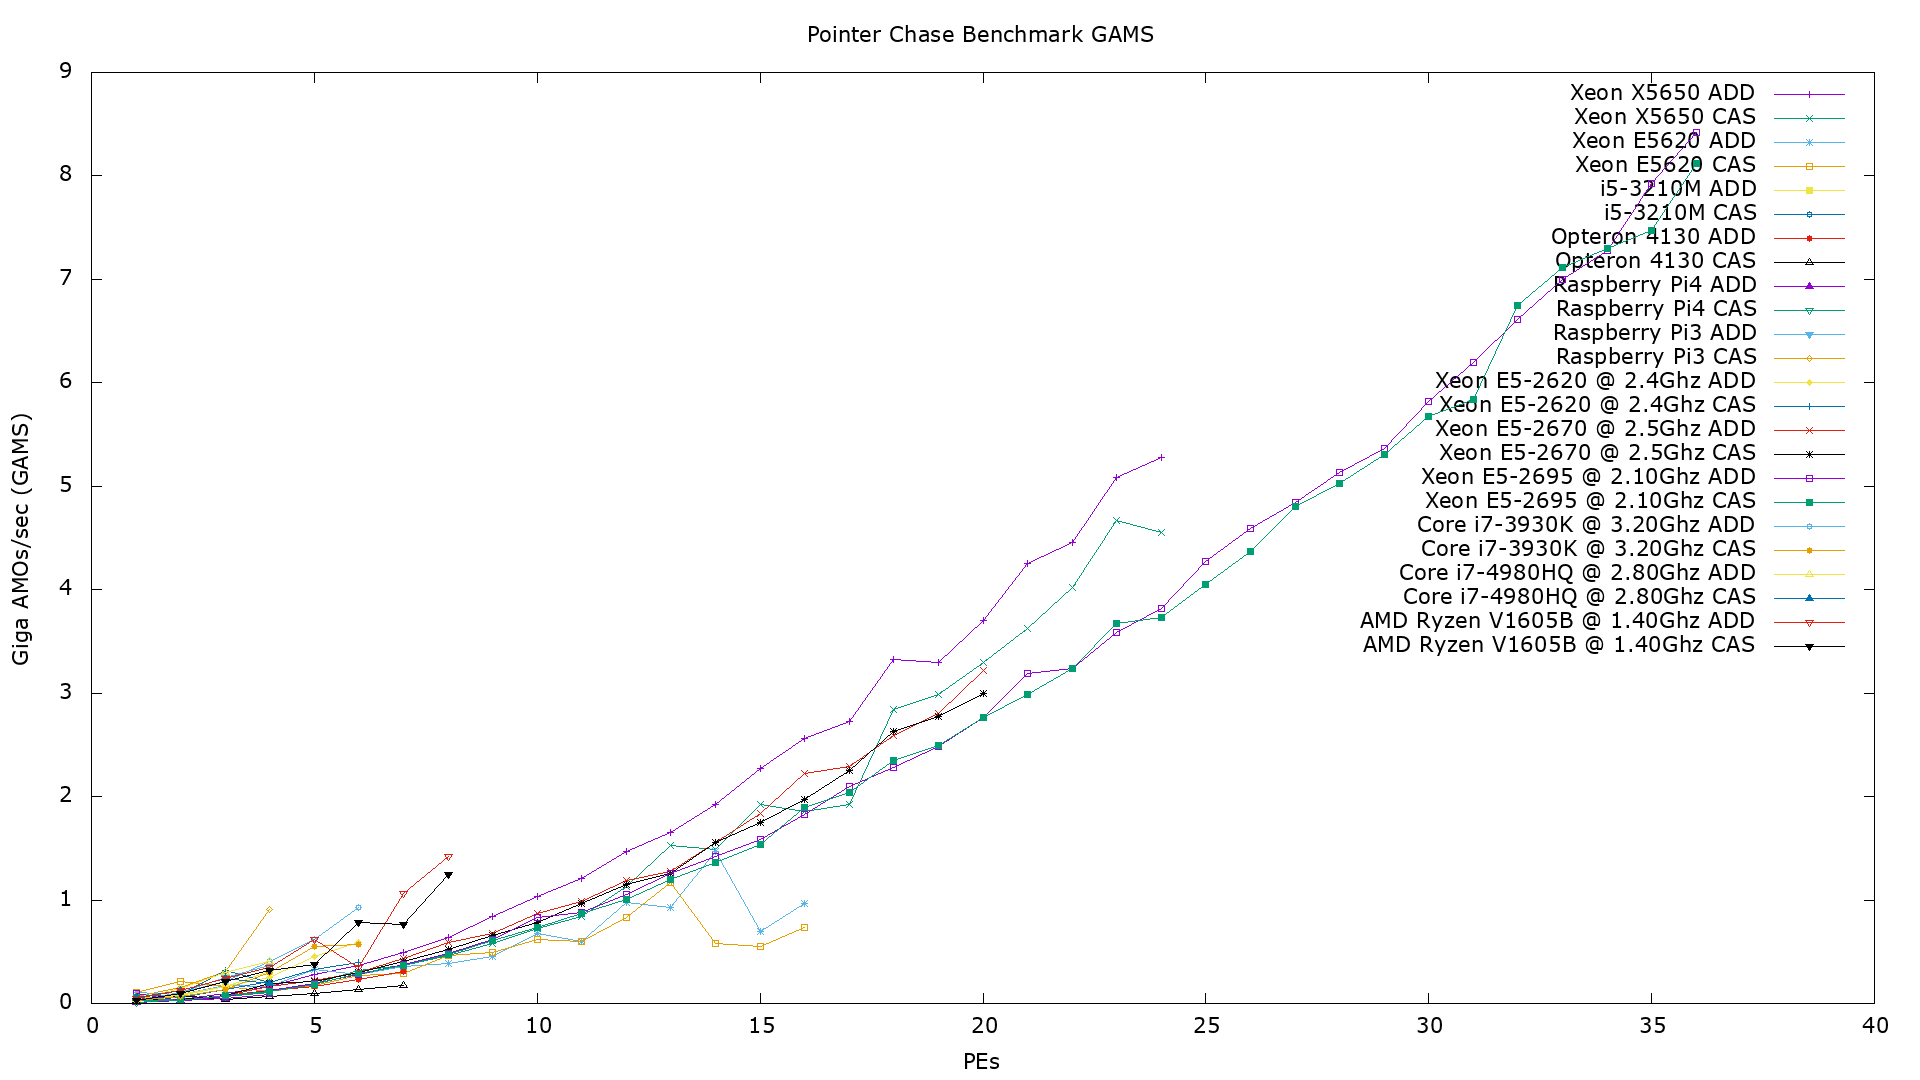
\includegraphics[width=3.5in]{figures/PTRCHASE_GAMS.png}
\caption{Pointer Chase Benchmark GAMS}
\label{fig:ptrchase_gams}
\end{figure}

\begin{figure}[!t]
\centering
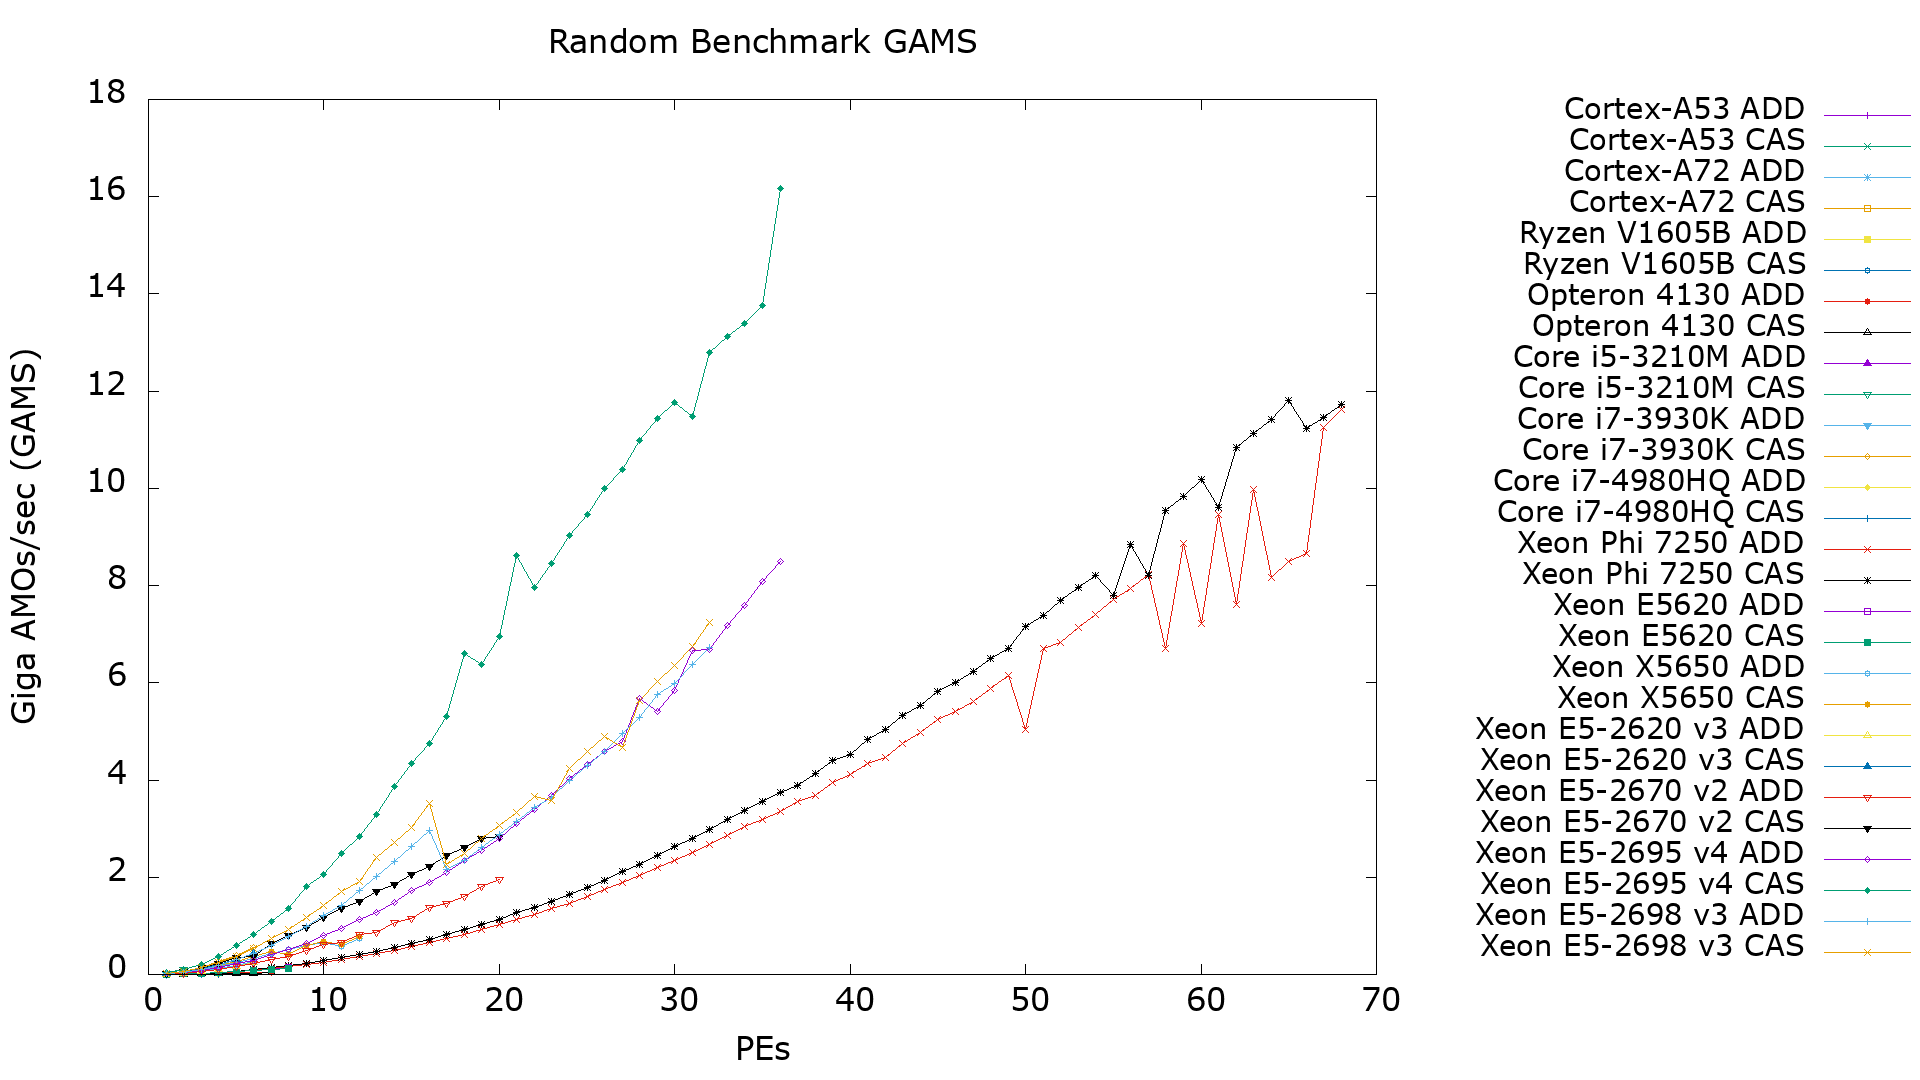
\includegraphics[width=3.5in]{figures/RAND_GAMS.png}
\caption{Random Benchmark GAMS}
\label{fig:rand_gams}
\end{figure}

\begin{figure}[!t]
\centering
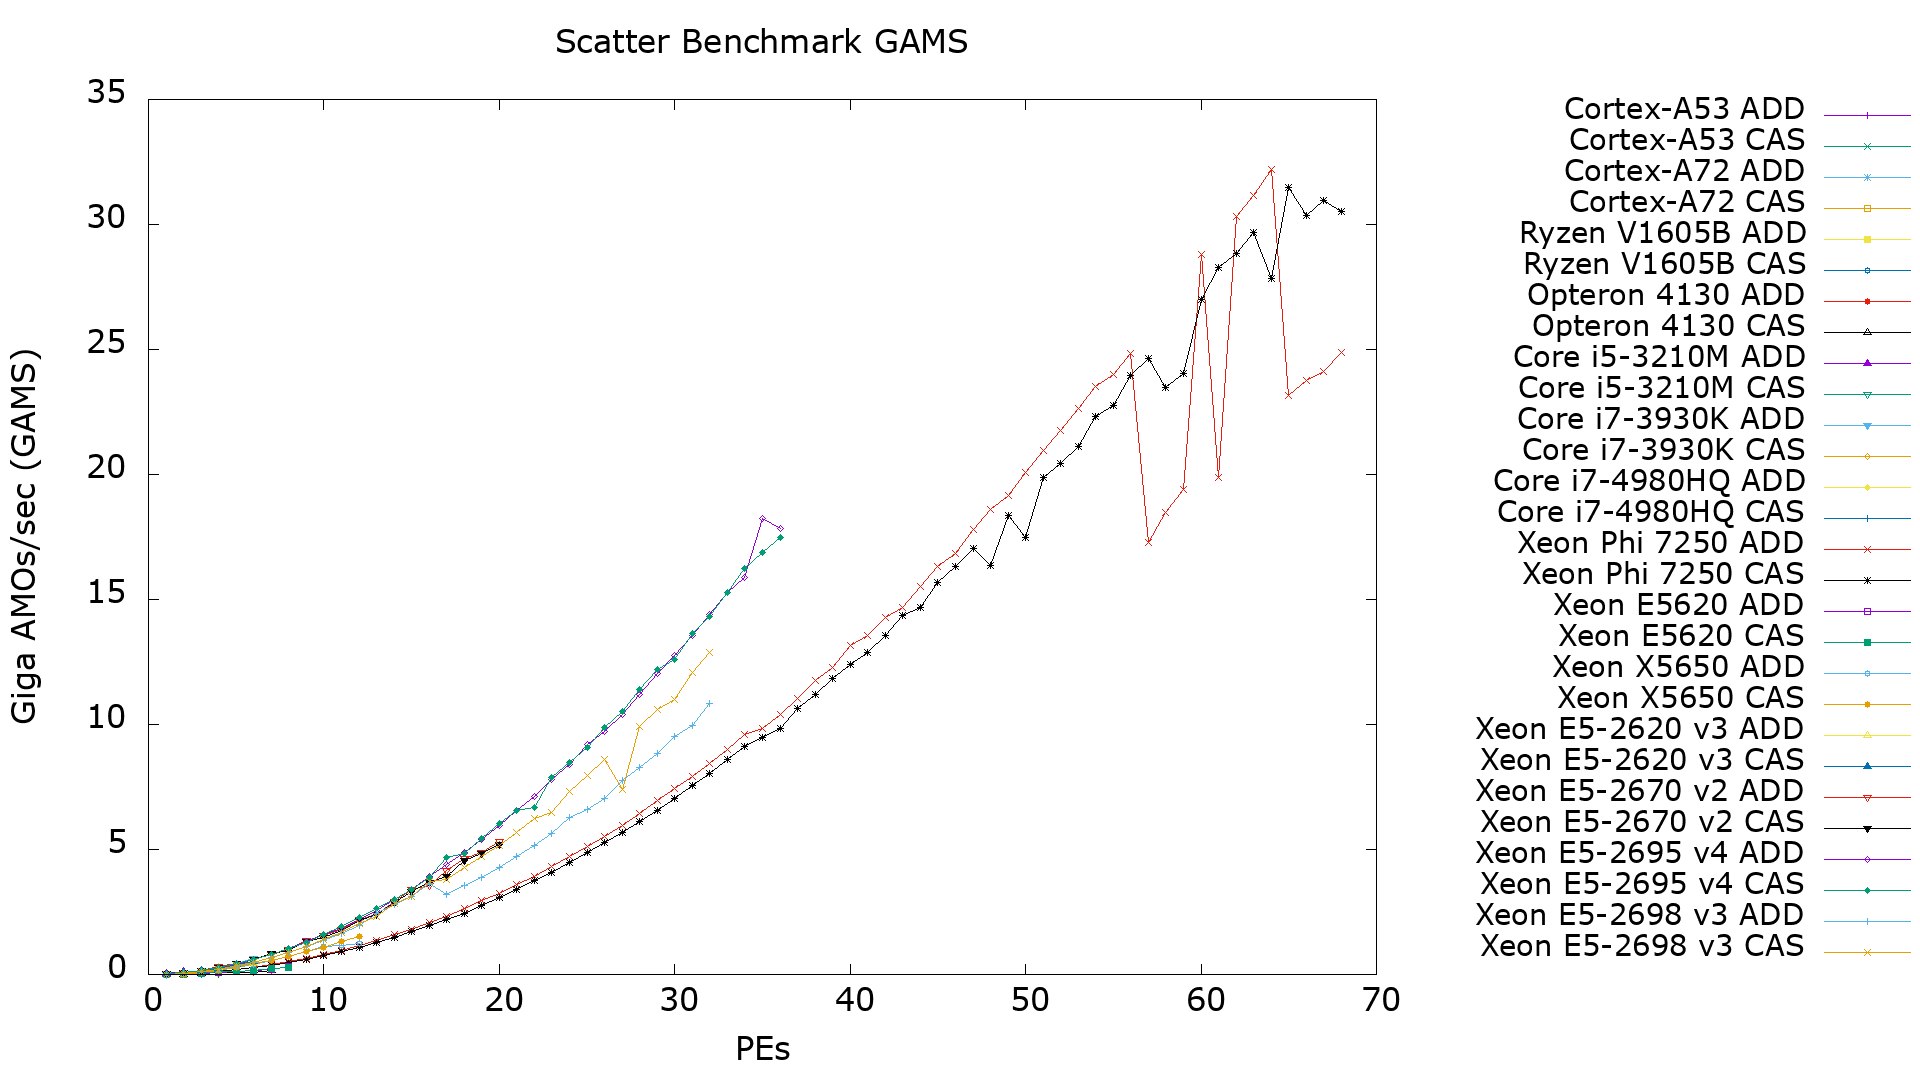
\includegraphics[width=3.5in]{figures/SCATTER_GAMS.png}
\caption{Scatter Benchmark GAMS}
\label{fig:scatter_gams}
\end{figure}

\begin{figure}[!t]
\centering
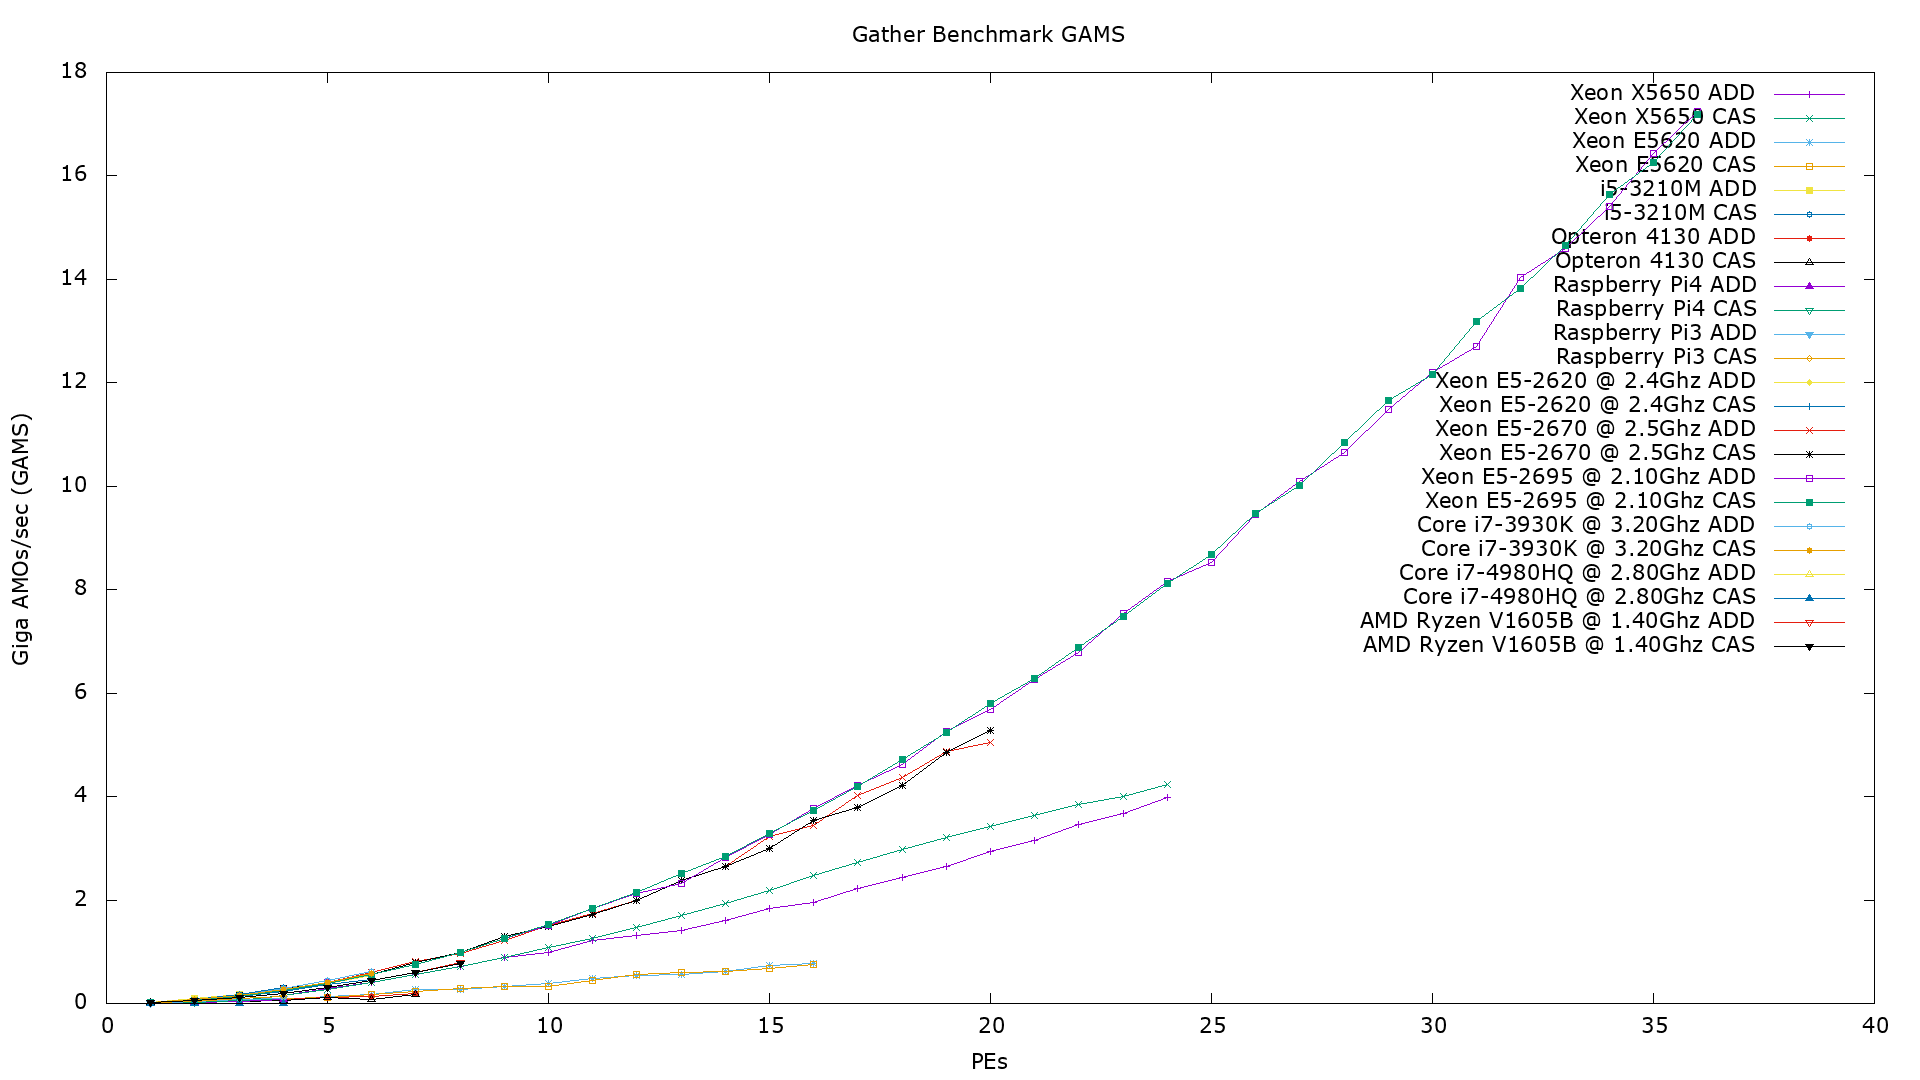
\includegraphics[width=3.5in]{figures/GATHER_GAMS.png}
\caption{Gather Benchmark GAMS}
\label{fig:gather_gams}
\end{figure}

\begin{figure}[!t]
\centering
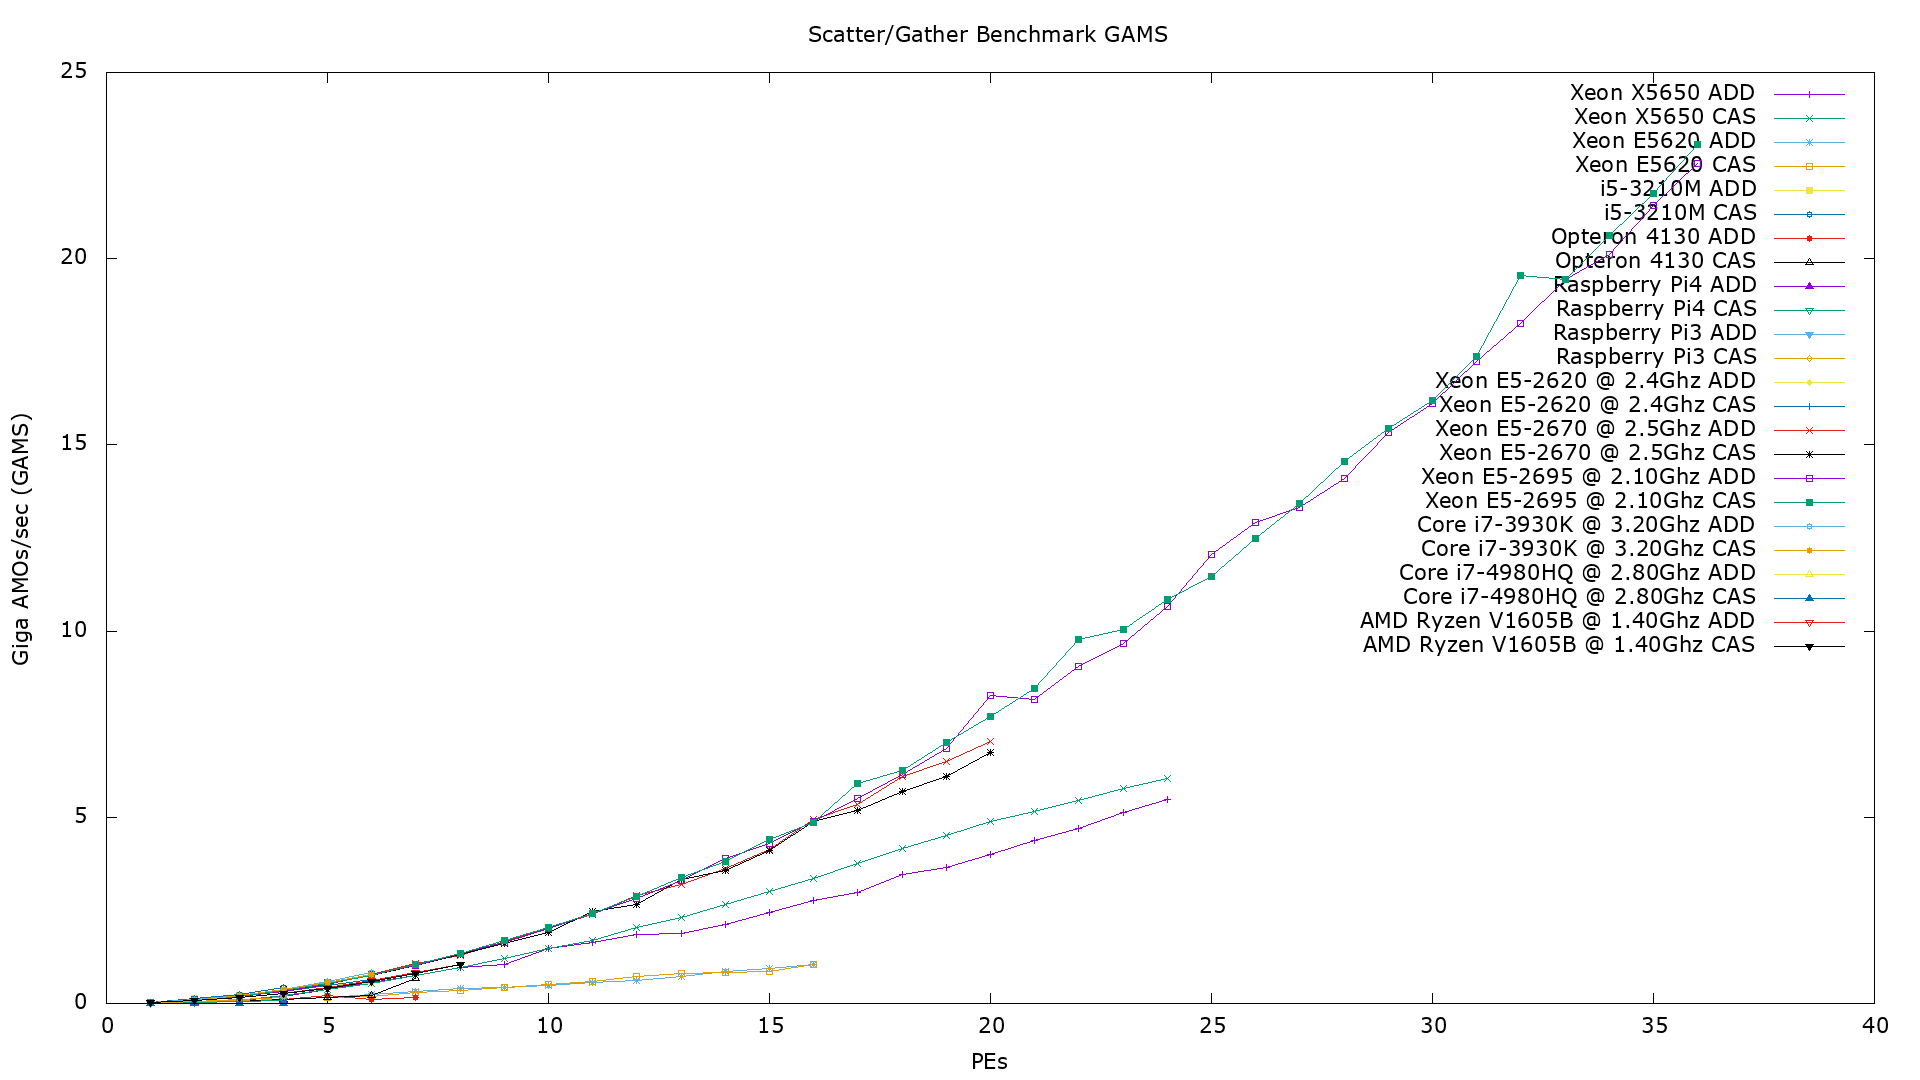
\includegraphics[width=3.5in]{figures/SG_GAMS.png}
\caption{Scatter/Gather Benchmark GAMS}
\label{fig:sg_gams}
\end{figure}

\begin{figure}[!t]
\centering
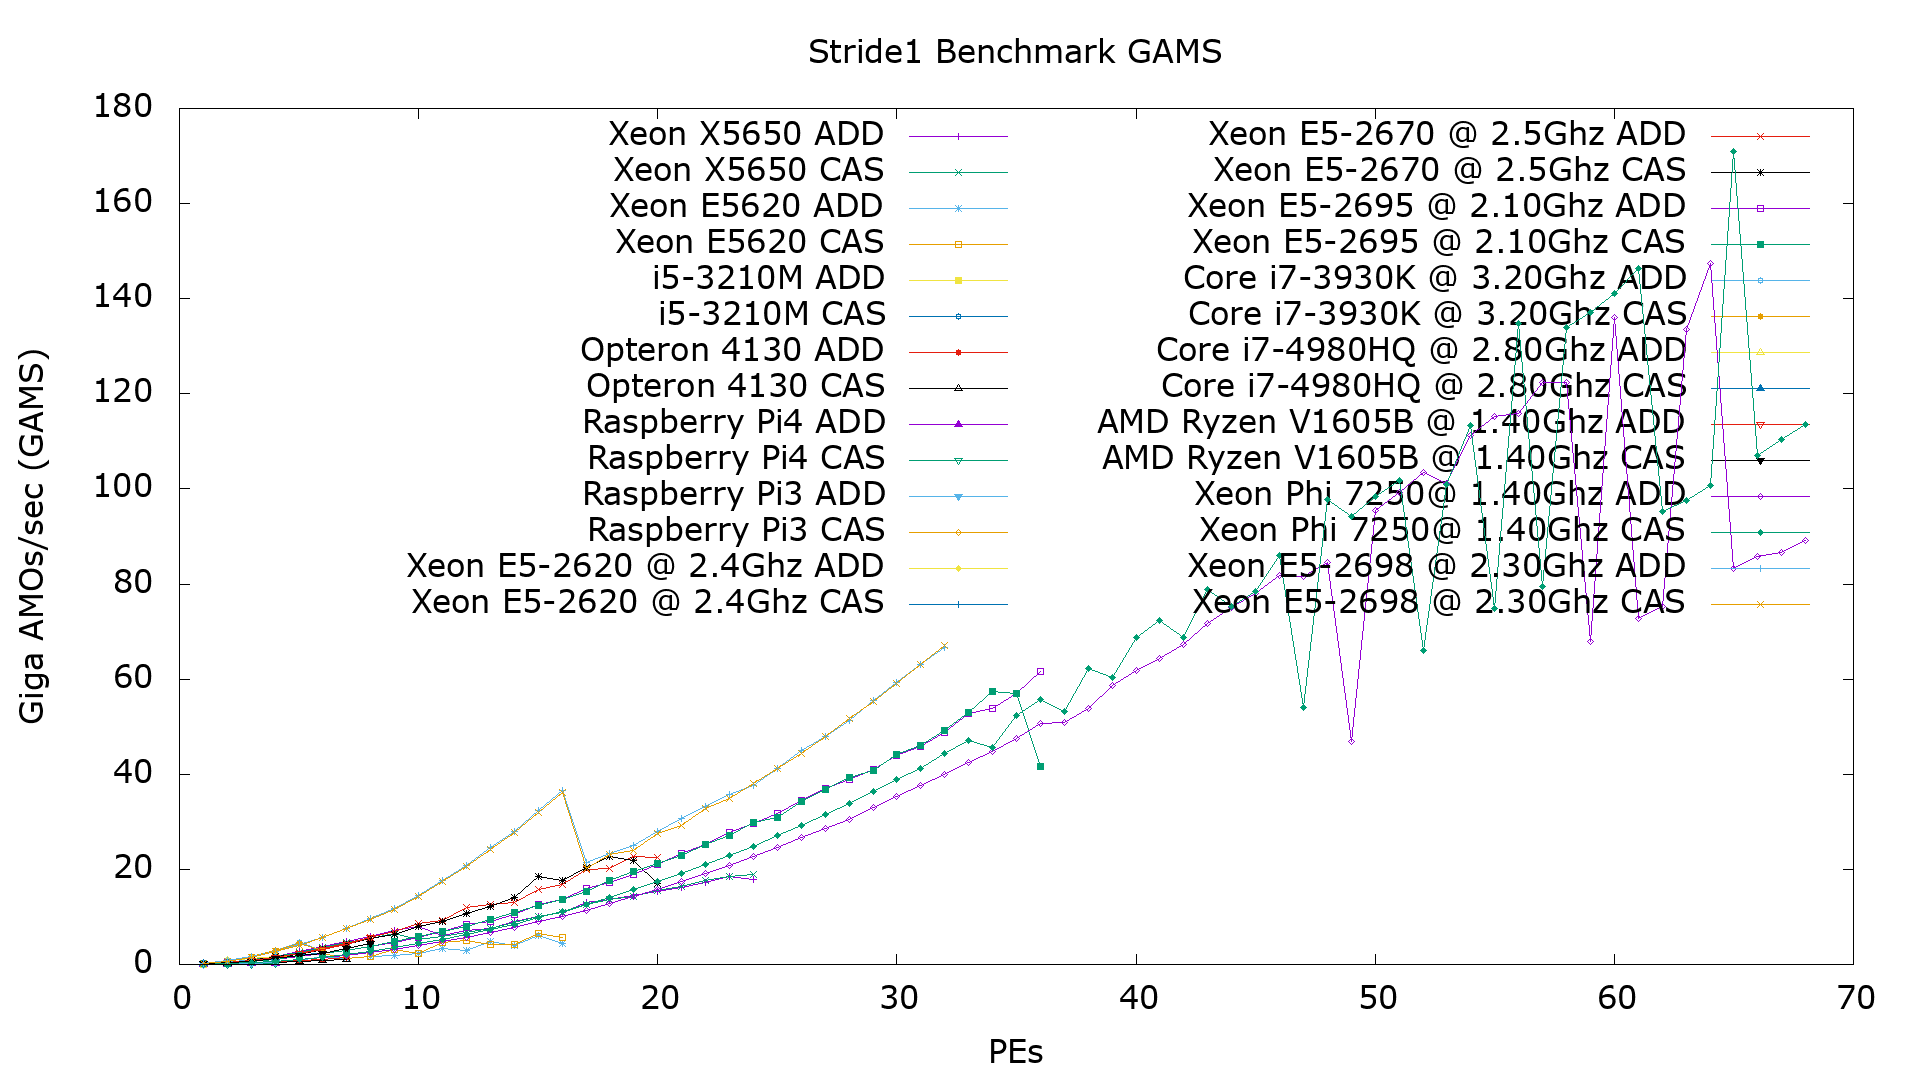
\includegraphics[width=3.5in]{figures/STRIDE1_GAMS.png}
\caption{Stride-1 Benchmark GAMS}
\label{fig:s1_gams}
\end{figure}

\begin{figure}[!t]
\centering
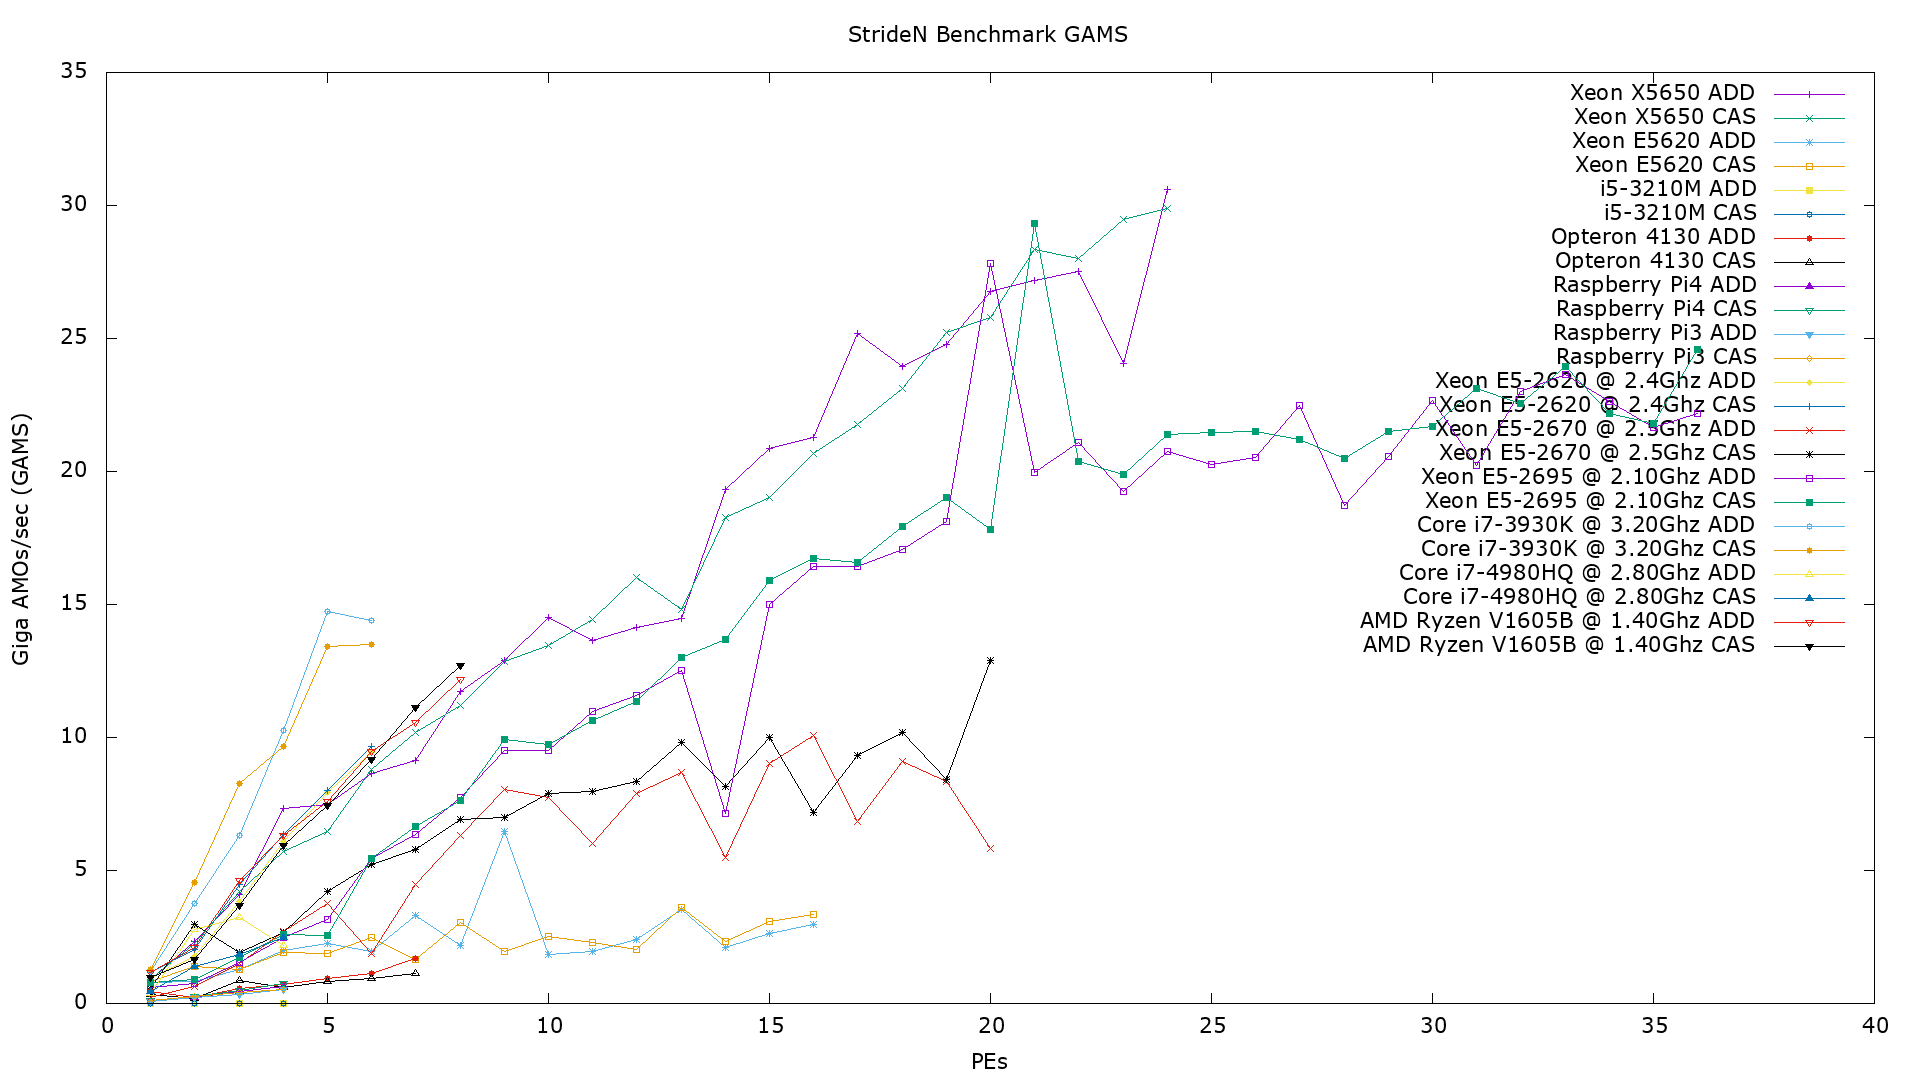
\includegraphics[width=3.5in]{figures/STRIDEN_GAMS.png}
\caption{Stride-N Benchmark GAMS}
\label{fig:sn_gams}
\end{figure}